\section{Hypertranscendence of the conjugacy}
\label{a:sec:ht}
This section makes the obstruction precise and delimits exactly what it does and does not assert. The logical skeleton is short. First, every elementary function satisfies an algebraic differential equation. Second, differential algebraicity survives compositional inversion. Third, by a theorem of Becker and Bergweiler, a solution of Schr\"oder's equation for a rational map of degree at least two can be differentially algebraic only when the underlying fixed point is \emph{repelling}. Fourth, for $r\in(0,1)$ the fixed point $0$ of $f_r$ is attracting. Hypertranscendence of $\psi_r$ for every subcritical parameter follows at once---with no exceptional cases to exclude, because the attracting window contains no candidates at all. We then explain, with equal care, why this theorem does \emph{not} by itself settle the status of the individual numbers $A(p_0)$ or of the map $p\mapsto A(p)$, and we record the numerical evidence bearing on those.

\subsection{Differential algebraicity, hypertranscendence, elementarity}

\begin{definition}[differentially algebraic; hypertranscendental]
\label{a:def:da}
A function $g$, holomorphic on a domain (or a formal power series), is \emph{differentially algebraic over $\mathbb{C}(z)$} if there exists a non-zero polynomial $P$ in $n+2$ variables, for some $n\ge0$, with
\[
P\bigl(z,\,g(z),\,g'(z),\,\dots,\,g^{(n)}(z)\bigr)\equiv 0 .
\]
Otherwise $g$ is \emph{differentially transcendental}, or \emph{hypertranscendental}.
\end{definition}

Two closure facts make this the right notion for our purpose.

\begin{lemma}[elementary $\Rightarrow$ differentially algebraic]
\label{a:lem:elem-da}
Every elementary function in the Liouville sense --- any function reachable from $\mathbb{C}(z)$ by a finite tower of algebraic operations, exponentials and logarithms --- is differentially algebraic. Consequently a hypertranscendental function is not elementary.
\end{lemma}

\begin{proof}[Proof sketch]
Each storey of a Liouvillian tower preserves differential algebraicity: algebraic extensions do so by elimination; if $g$ is differentially algebraic then so are $e^{g}$ and $\log g$, their defining first-order relations combining with the equation for $g$; and the class is closed under field operations and composition. These closure properties are classical; see Rubel's survey \cite{Rubel1989}.
\end{proof}

\begin{lemma}[closure under compositional inversion]
\label{a:lem:inv-da}
Let $g$ be holomorphic near $0$ with $g(0)=0$ and $g'(0)\neq0$, and let $g^{-1}$ denote its local compositional inverse. Then $g$ is differentially algebraic over $\mathbb{C}(z)$ if and only if $g^{-1}$ is (Moore \cite{Moore1896}; see also Boshernitzan--Rubel \cite{BoshernitzanRubel1986}).
\end{lemma}

\Cref{a:lem:inv-da} matters because the literature states Schr\"oder-equation results in two equivalent but opposite conventions, and conflating them is an easy way to misquote a theorem. Our $\psi_r$ is the \emph{linearising coordinate}: $\psi_r(f_r(z))=r\,\psi_r(z)$. The function classified by Becker and Bergweiler (and by Ritt before them) is the \emph{linearising parametrisation} $\varphi_r=\psi_r^{-1}$, which satisfies
\begin{equation}
\label{a:eq:schroder-param}
\varphi_r(r\,t)=f_r\bigl(\varphi_r(t)\bigr),
\qquad
\varphi_r(0)=0,\quad \varphi_r'(0)=1 .
\end{equation}
By \Cref{a:lem:inv-da}, hypertranscendence of either function transfers to the other.

\subsection{The Becker--Bergweiler theorem, stated precisely}

The result we need is the 1995 classification of differentially algebraic Schr\"oder functions \cite{Becker1995}; we quote it in the form given in Fernandes' survey of the Schr\"oder, B\"ottcher and Abel equations \cite[Thm~3.1]{Fernandes2021}.

\begin{theorem}[Becker--Bergweiler \cite{Becker1995}; as restated in {\cite[Thm~3.1]{Fernandes2021}}]
\label{a:thm:BB-main}
Let $R$ be a rational map of degree at least two with $R(0)=0$ and multiplier $s=R'(0)$, where $s\neq0$ and $s$ is not a root of unity (for $|s|=1$ the Schr\"oder function is understood as a formal series). Let $\varphi$, normalised by $\varphi(0)=0$ and $\varphi'(0)=1$, solve $\varphi(st)=R(\varphi(t))$. If $\varphi$ is differentially algebraic over $\mathbb{C}(t)$, then:
\begin{enumerate}[label=\textup{(\roman*)}]
\item the fixed point $0$ is \emph{repelling}, $|s|>1$; and
\item $\varphi$ is a M\"obius transformation of one of
\[
\exp(\alpha t^{\rho}),
\qquad
\cos(\alpha t^{\rho}+\beta),
\qquad
\wp(\alpha t^{\rho}+\beta),\ \wp^{2},\ \wp^{3},\ \wp'(\alpha t^{\rho}+\beta),
\]
where $\wp$ is a Weierstrass function, $\rho\in\mathbb{Q}$ is such that the function concerned is meromorphic on $\mathbb{C}$, $\alpha\neq0$, and $\beta$ is a fraction of a period. Correspondingly $R$ is M\"obius-conjugate to $z^{\pm d}$, to $\pm T_d$ (Chebyshev), or to a Latt\`es map.
\end{enumerate}
\end{theorem}

\begin{remark}[lineage and independent corroboration]
\label{a:rem:lineage}
For $|s|>1$ --- the Poincar\'e-function case --- the classification goes back to Ritt in 1926 \cite{Ritt1926}; Becker and Bergweiler completed the picture for the three classical functional equations at once, and Bergweiler's later account with Aschenbrenner \cite{AschenbrennerBergweiler2015} assigns the exceptional list explicitly to the repelling case. Di~Vizio and Fernandes \cite{DiVizioFernandes2021} have given an independent difference-Galois proof of Ritt's theorem; notably, their Theorems~1.2 and~4.2 assume only that $s$ is neither zero nor a root of unity --- no condition $|s|>1$ --- and show that any differentially algebraic solution of $y(R(x))=s\,y(x)$ (our $\psi$-convention, with no inversion needed) must already satisfy a first-order equation of Ritt type $(y')^{\rho}=B(x)\,y^{\,j}$. The structure underlying \Cref{a:thm:BB-main} therefore does not hang on a single paper.
\end{remark}

\subsection{Hypertranscendence throughout the subcritical window}

\begin{theorem}[no exceptional parameters in $(0,1)$]
\label{a:thm:main-ht}
For every $r\in(0,1)$, the Koenigs function $\psi_r$ of $f_r(z)=rz(1-z)$ at $0$ is hypertranscendental over $\mathbb{C}(z)$: it satisfies no algebraic differential equation. In particular, $\psi_r$ is not an elementary function.
\end{theorem}

\begin{proof}
Fix $r\in(0,1)$. The map $f_r$ is rational of degree two, fixes $0$, and its multiplier $s=f_r'(0)=r$ satisfies $0<s<1$; the hypotheses of \Cref{a:thm:BB-main} hold, with $0$ attracting. Suppose, for contradiction, that $\psi_r$ were differentially algebraic. Its local inverse $\varphi_r=\psi_r^{-1}$ solves the parametrisation form \eqref{a:eq:schroder-param} with the stated normalisation, and by \Cref{a:lem:inv-da} it would be differentially algebraic too. \Cref{a:thm:BB-main}(i) would then force $|r|>1$, contradicting $r\in(0,1)$. Hence $\psi_r$ is hypertranscendental, and non-elementarity follows from \Cref{a:lem:elem-da}.
\end{proof}

\begin{remark}[the exceptional set inside the window is empty, not merely avoided]
\label{a:rem:empty}
An earlier form of this argument reasoned through the parameter plane: the affine conjugacy $c(r)=(2r-r^{2})/4$ of \Cref{a:lem:affine} sends $r\in(0,1)$ to $c\in(0,\tfrac14)$, which avoids the exceptional quadratic parameters $c=0$ (reached at $r=2$) and $c=-2$ (reached at $r=4$, and also at $r=-2$). That observation is true but logically superfluous, and it invites a question it cannot answer --- \emph{is the exceptional list, restricted to the window, complete?} The route through \Cref{a:thm:BB-main}(i) dissolves the question: the exceptional Schr\"oder functions exist only over \emph{repelling} fixed points, so the attracting window contains no candidates whatsoever, and no enumeration of exceptional parameters is required. Consistently, the classical elementary cases of \cref{a:app:integrable} have multipliers $2$ and $4$ at the linearised fixed point --- both repelling: they are Poincar\'e-type linearisations, and neither can be pressed into service for $r\in(0,1)$.
\end{remark}

\begin{figure}[H]
\centering
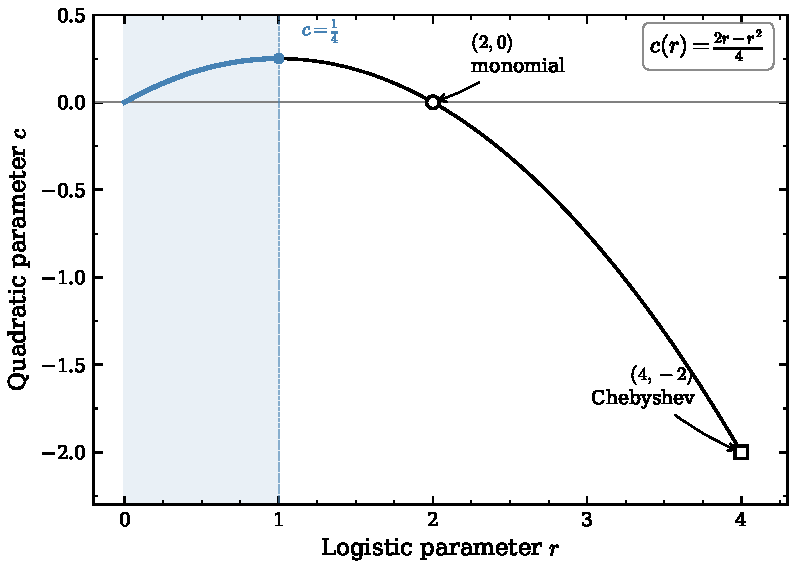
\includegraphics[width=0.72\textwidth]{figures/IMG_ch3/figure1_parameter_conjugacy.pdf}
\caption{Parameter correspondence $c(r)=(2r-r^2)/4$. The segment $r\in(0,1)$ maps to $c\in(0,\tfrac14)$, disjoint from the integrable values $c\in\{0,-2\}$. In the light of \Cref{a:rem:empty} this picture is a consistency check rather than the proof: the exceptional linearisations live over repelling fixed points, which the attracting window excludes outright.}
\label{a:fig:c-of-r}
\end{figure}

\begin{remark}[germ versus basin]
\label{a:rem:basin}
\Cref{a:thm:main-ht} concerns $\psi_r$ as an analytic function; the quantity $A(p)=2\psi_r(\tfrac12)$ of \eqref{a:eq:AeqKoenigs} uses its extension to the real basin of attraction, since for $p\ge\tfrac13$ the point $\tfrac12$ lies outside the disc on which Koenigs' series is guaranteed to converge (radius $(1-r)/r$). The extension is by finitely many applications of the functional equation,
\[
\psi_r(w)=r^{-N}\,\psi_r\bigl(f_r^{\circ N}(w)\bigr)
\quad\text{for $N$ large enough that $f_r^{\circ N}(w)$ enters the germ,}
\]
and an algebraic differential equation, if one held on any subdomain, would persist under this analytic continuation. Hypertranscendence of the germ and of the basin extension are therefore equivalent statements, and the identity \eqref{a:eq:AeqKoenigs} is unaffected.
\end{remark}

\begin{figure}[H]
\centering
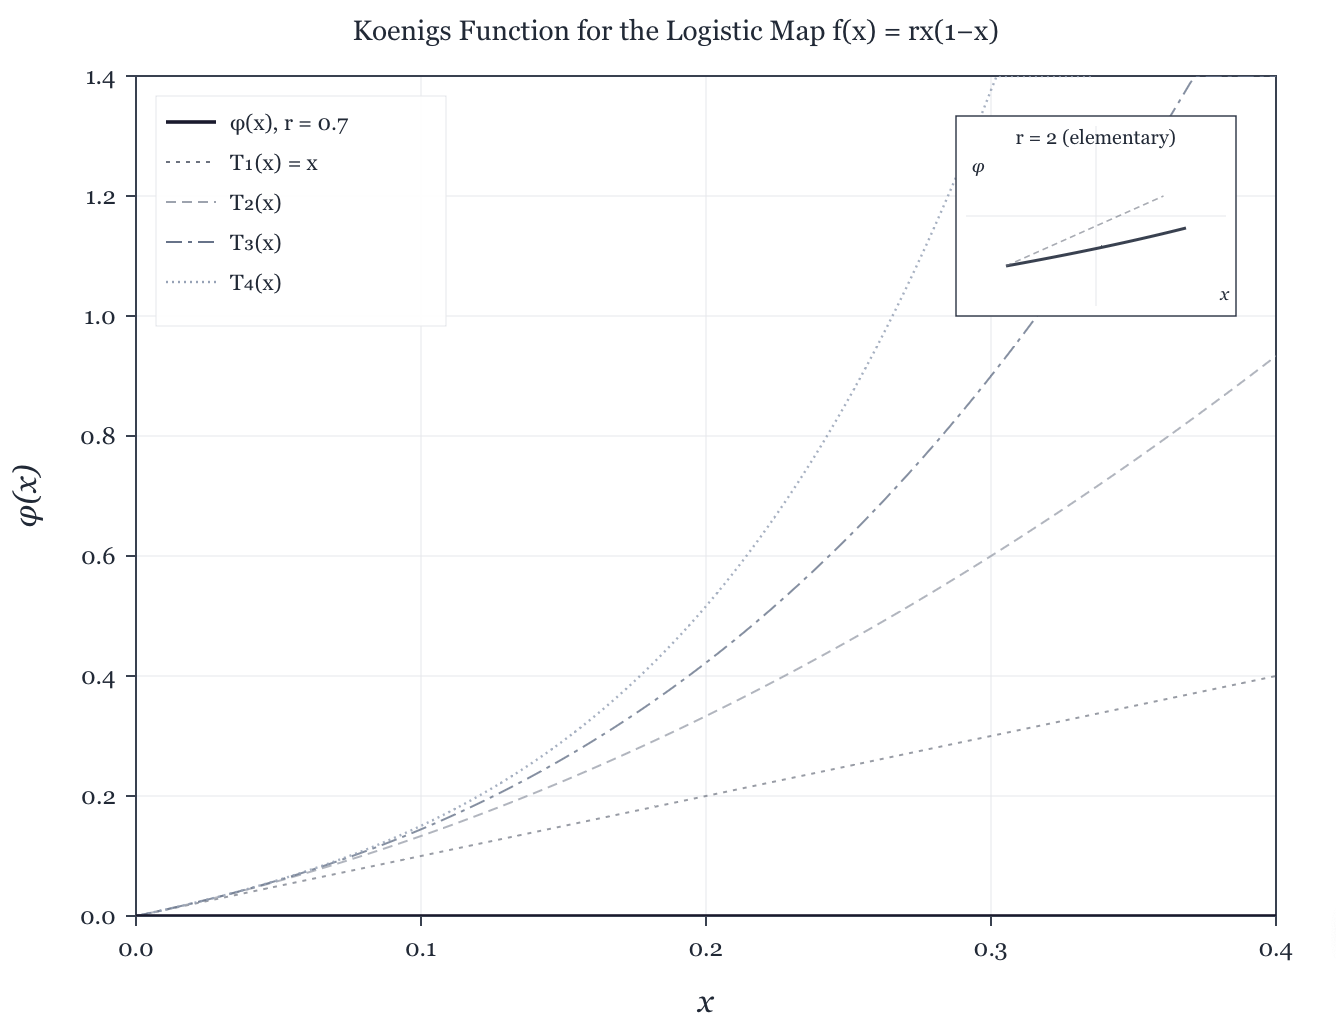
\includegraphics[width=0.72\textwidth]{figures/figure3_numerical_koenigs.png}
\caption{Numerical approximation of a Koenigs function for a logistic multiplier in $(0,1)$, with low-order Taylor polynomials near the origin. Elementary closed forms exist only for exceptional multipliers outside this range (\cref{a:app:integrable}).}
\label{a:fig:koenigs-numeric}
\end{figure}
